\documentclass[10pt]{article}
\usepackage[margin=0.75in]{geometry}
\usepackage{graphicx,booktabs,amsmath,hyperref}
\hypersetup{colorlinks=true,urlcolor=blue}
\title{HTT observational applications: conditional results from retained products}
\author{HTT observational research}\date{14 October 2026}
\begin{document}\maketitle
\begin{abstract}
We executed retained-product observational diagnostics, a selected 24-group CF4
scenario posterior and latent predictive image, and a joint Union3--DESI compressed
distance posterior. Scientific interpretation remains conditional on the declared
processing, selection, covariance and model assumptions. No physical shear, global
tilt, native Bianchi family, or physical MES admission follows.
\end{abstract}
\section{Joint distance result}
Union3 has 22 compressed nodes, not 22 independent supernovae. One DESI BGS
$q_{\rm iso}$ summary enters once. In the flat late-time matter--Lambda scenario,
$E(z)^2=\Omega_m(1+z)^3+1-\Omega_m$ and $I(z)=\int_0^z du/E(u)$.
We analytically integrate a common magnitude offset $M\sim N(43,5^2)$.
Proper priors are $\Omega_m\sim U(.01,.99)$ and $H_0r_d\sim U(5000,20000)$ km/s.
The reference factorization scenario gives $\Omega_m=0.357456\pm0.027084$ and
$H_0r_d=9974.63\pm204.18$ km/s. It does not separate $H_0$ and $r_d$.
Five covariance scenarios $\rho=0,\pm.25,\pm.5$ preserve the released marginal
covariances. These are assumptions, not measured cross-covariances or posterior odds.
Orders128,256,512 close the declared quadrature criteria. The posterior image retains
all original 262144 node IDs and weights. Physical MES fields remain unavailable,
with unknown mass 1; imposed distance geometry is not measured zero anisotropy.
\section{Selected CF4 scenario}
For 24 SNIa-only grouped observations, $x=\log d_A$, $t=c\log(1+z_{\rm true})$,
$\mu=25+(5/\ln10)x+2(5/\ln10)t/c+\eta$.
A single shared zero point is integrated with the preselection law
$L=[\int p(\eta)\prod_i f_i d\eta]/[\int p(\eta)\prod_i Z_i d\eta]$.
The finite-box endpoint posterior has 2048 nodes and ESS1120.83.
The endpoint coefficient is not cosmological $H_0$.
Same-state $d_L=d_A(1+z_{\rm true})^2$ and repeated-measurement PPC give
exceedance 0.678020; this is not a uniform null p-value. Thirty-two frozen same-law
injections resolve; endpoint-H bias -0.357125 and RMSE 1.953703.
The interval study is finite conditional Gaussian-Wald calibration, not empirical
CF4 coverage. Population, velocity width, calibration and remainder are scenarios.
No certified remainder upper bound is obtained.
\section{Temperature and polarization}
SMICA tensor-family conditional rank is17/241; a joint 48-choice processing scan
has rank 63/241. Both procedures reuse the same sky and the same 300 paired simulations. Each has
disjoint training 60 and calibration 240 subsets, but the two results are not independent. No
improvement relative to historical p=.039 is inferred. Temperature quadrupole is not
physical shear, and residual ell1 is not a physical dipole.
BK18's actual 66 correlatedBB spectra in 9 bins give fixed-fiducial HL descriptor
$Q_{\rm HL}=545.104273$, with independent/native algebra parity. It is not a PTE,
normalized evidence or primordial-r fit. CLASS 200 unique-per-split noise pairs
produce a six-feature joint conditional rank 0.00621118; EE drives this maximum,
whereas the displayed BB components are near their noise means. Its independent
split-noise law is an approximation; signal leakage/systematics are not calibrated.
The first raw FFP10 pair closes six-transform spin2 linearity and signed cross-term
checks under two formal U encodings. Raw-product frame/convention/processing binding
remains HOLD; no ensemble or actual-data inference is made.
\section{Other retained products and limitations}
The ACT--Planck released joint lensing amplitude, its Planck marginal and the Planck
PR3 reference are overlapping products; they are not multiplied independently.
The source-qualified Planck PR3 corrected reference amplitude is $A_{PP}=1.009562\pm0.026253$. Its reference cosmology already includes Planck lensing; this is release consistency, not independent calibration. CMB marginalization has used primary CMB information and does not establish product independence.
Source-matched Planck/ACT/SPT spectrum residuals retain their reference, covariance
and foreground/calibration scope. BeyondPlanck mean maps are not independent skies.
COSMOS scans all released 784016 rows, including zero zfinal placeholders; retention
is not completeness or a galaxy-population law. Gaia fits 4756 selected frame sources
with 2x2 covariance blocks; upstream outcome selection prevents an independent physical
frame test. JWST/CCHP photometry, KiDS n(z), Union3 deletion and SDSS observer-box
controls retain their shared-source and conditional assumptions.
\section{Provenance and review}
Exact generating result files, code/input identities, fixed assumptions, figures and
review scopes accompany this report in report.json and figure\_inventory.json.
Requested author/reviewer settings are separate from observed runtime UNKNOWN.
Prior scoped results and upper proofs are reused. Physical joint-model and external
native atlas dependencies remain gated. See the Korean report and RETURN for exact
missing inputs and resume commands. Publication is not scientific admission.
\paragraph{Primary source context.}
\href{https://github.com/rubind/union3_release}{Union3 release};
\href{https://arxiv.org/abs/1807.06208}{Planck component separation};
\href{https://arxiv.org/abs/1807.06210}{Planck lensing};
\href{https://github.com/ACTCollaboration/act_dr6_lenslike}{ACT lensing software};
\href{https://arxiv.org/abs/2110.00483}{BICEP/Keck XIII};
\href{https://lambda.gsfc.nasa.gov/product/class/}{CLASS release};
\href{https://cosmos2025.iap.fr/catalog.html}{COSMOS-Web};
\href{https://arxiv.org/abs/2204.12574}{Gaia celestial frame}.

\clearpage\begin{figure}[p]\centering
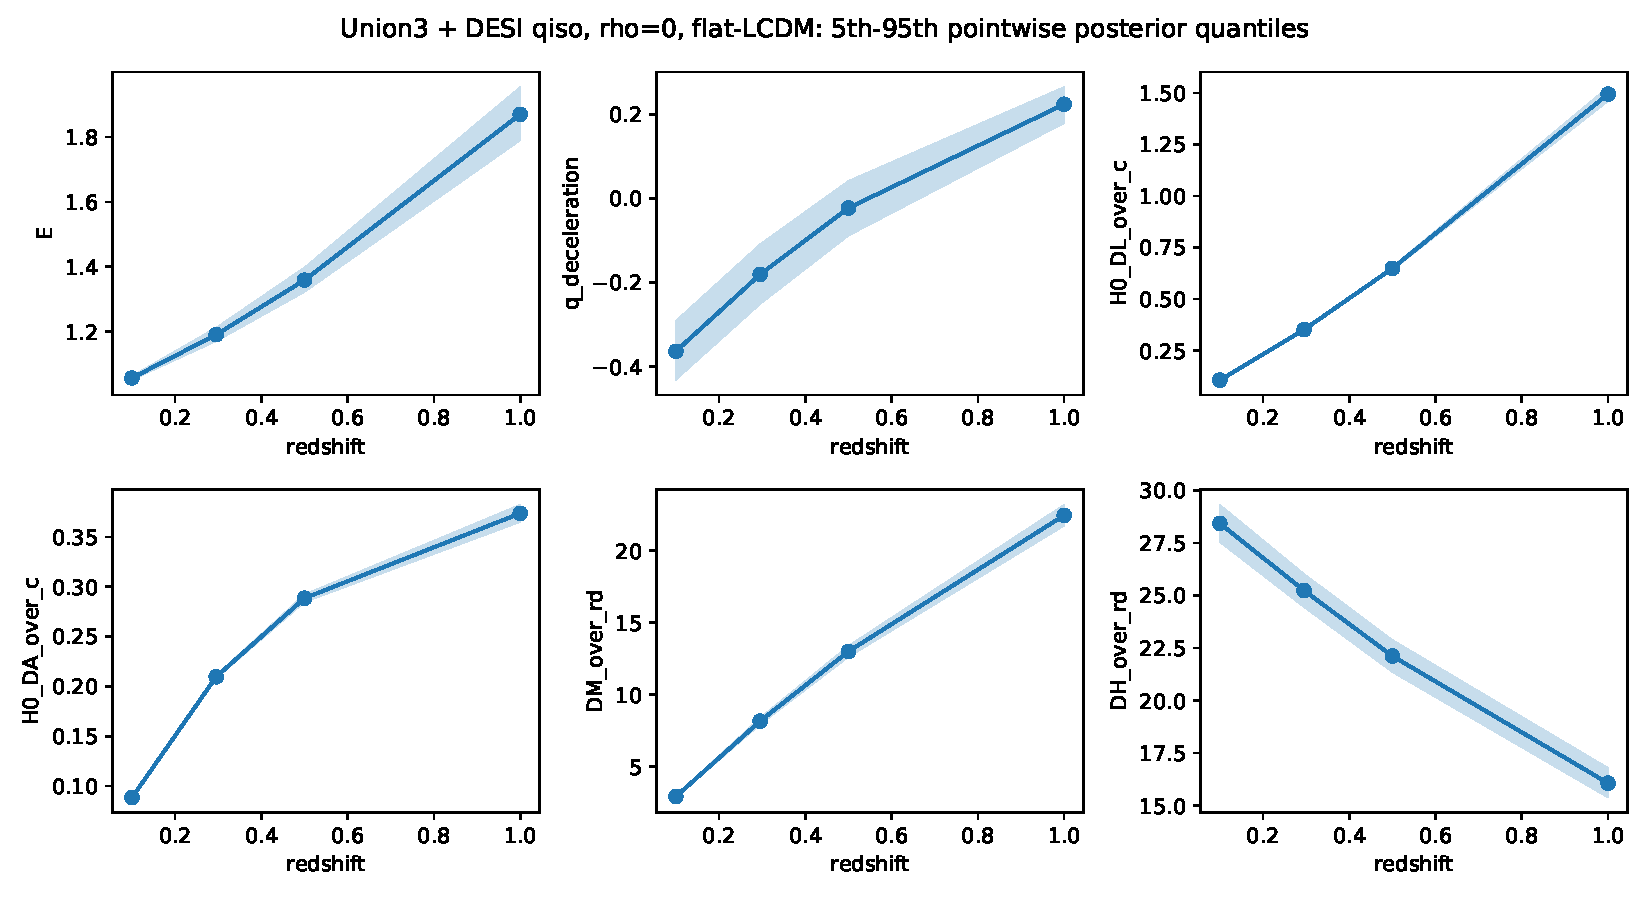
\includegraphics[width=\linewidth,height=.70\textheight,keepaspectratio]{../posterior/legacy_distance_image.pdf}
\caption{Same posterior rho=0 flat-LCDM distance functions; pointwise5/95\% quantiles; physical MES unavailable}
\end{figure}

\clearpage\begin{figure}[p]\centering
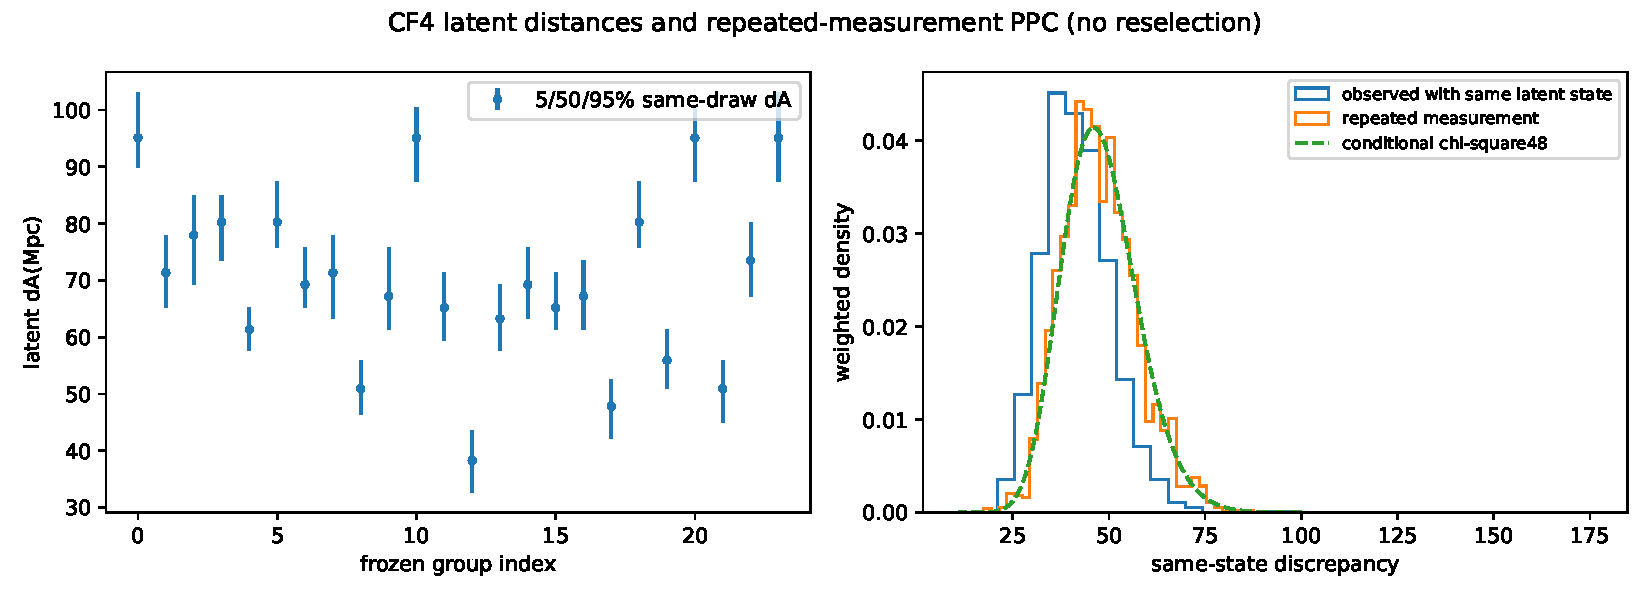
\includegraphics[width=\linewidth,height=.70\textheight,keepaspectratio]{../cf4/latent_v1/latent_ppc.pdf}
\caption{Same posterior latent dA and repeated measurement PPC, without reselection; conditional selected scenario}
\end{figure}

\clearpage\begin{figure}[p]\centering
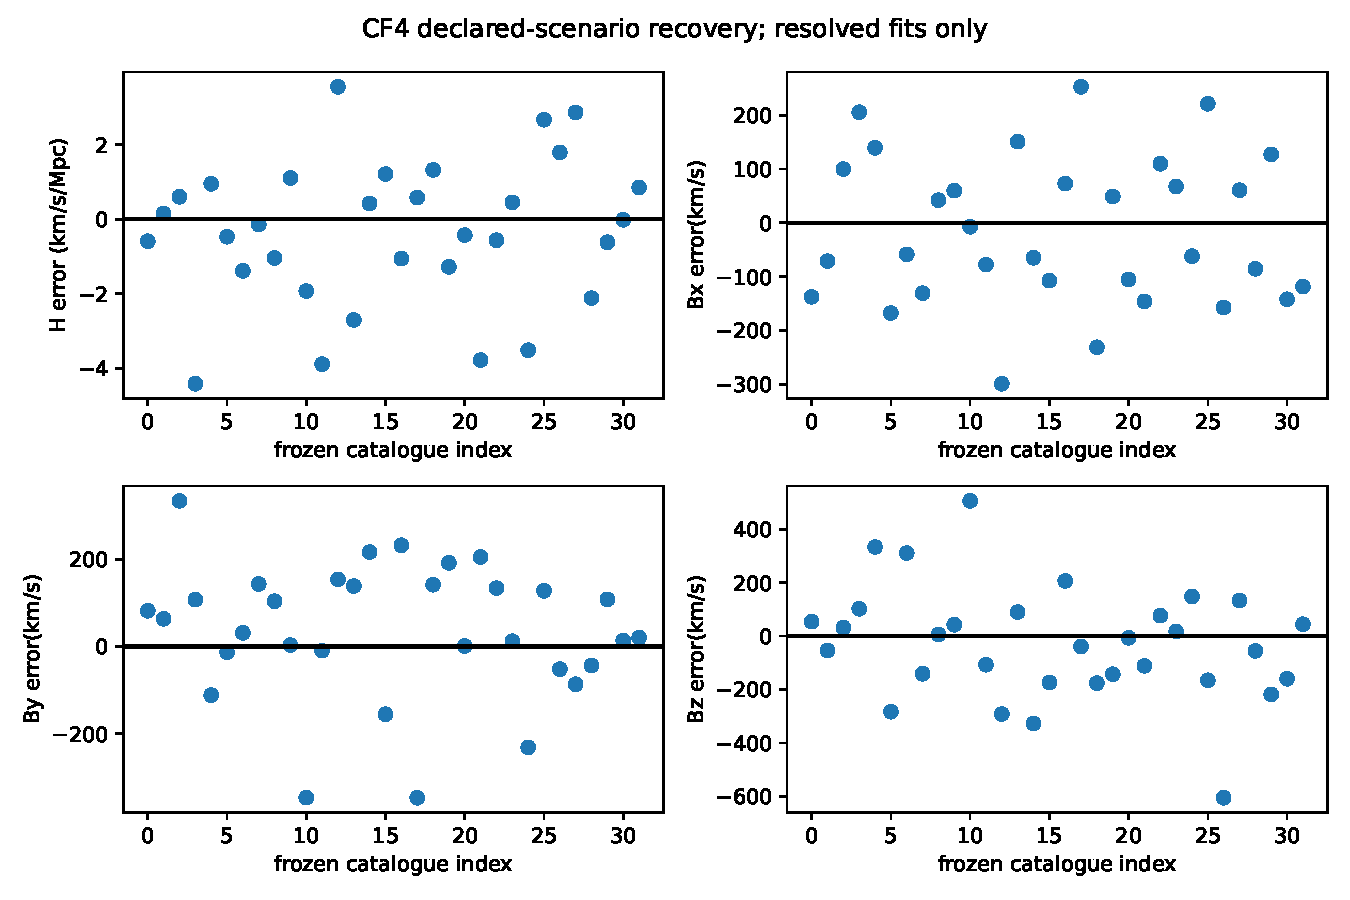
\includegraphics[width=\linewidth,height=.70\textheight,keepaspectratio]{../cf4/injection_v1/recovery.pdf}
\caption{32 conditional selected scenario injections, not empirical CF4 coverage}
\end{figure}

\clearpage\begin{figure}[p]\centering
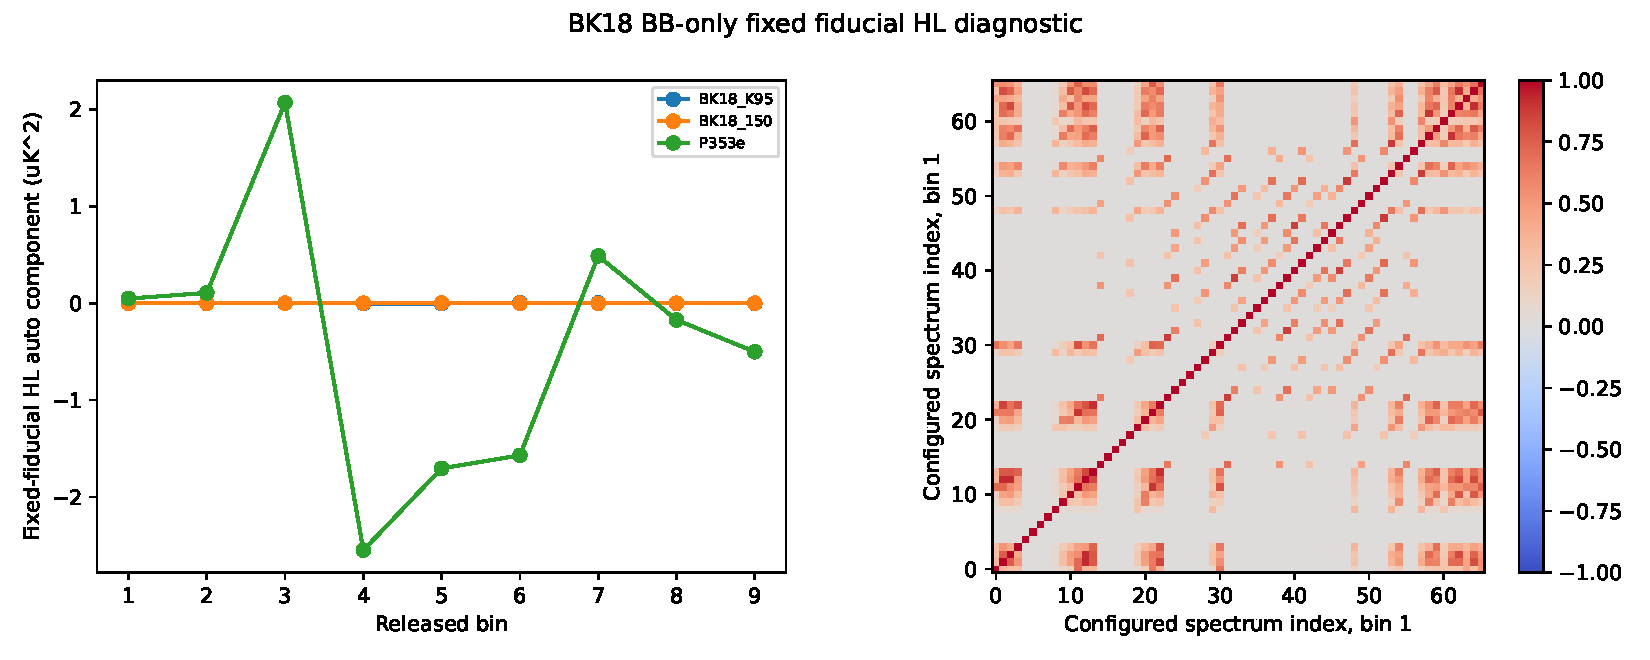
\includegraphics[width=\linewidth,height=.70\textheight,keepaspectratio]{../bk18_fixed_fiducial_v1/diagnostic.pdf}
\caption{BK18 correlated fixed fiducial HL descriptor; no PTE or r fit}
\end{figure}

\clearpage\begin{figure}[p]\centering
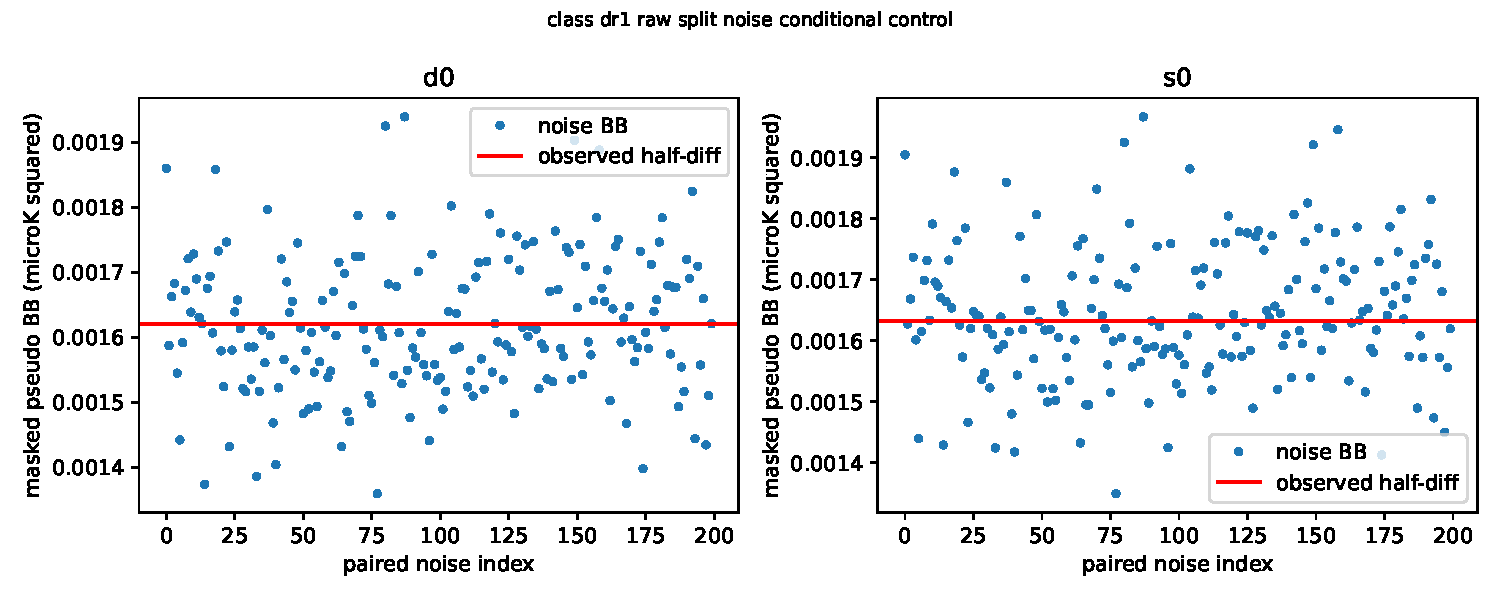
\includegraphics[width=\linewidth,height=.70\textheight,keepaspectratio]{../class_noise_v1/diagnostic.pdf}
\caption{CLASS BB component only; joint six feature rank driven by EE; independent split-noise approximation}
\end{figure}

\clearpage\begin{figure}[p]\centering
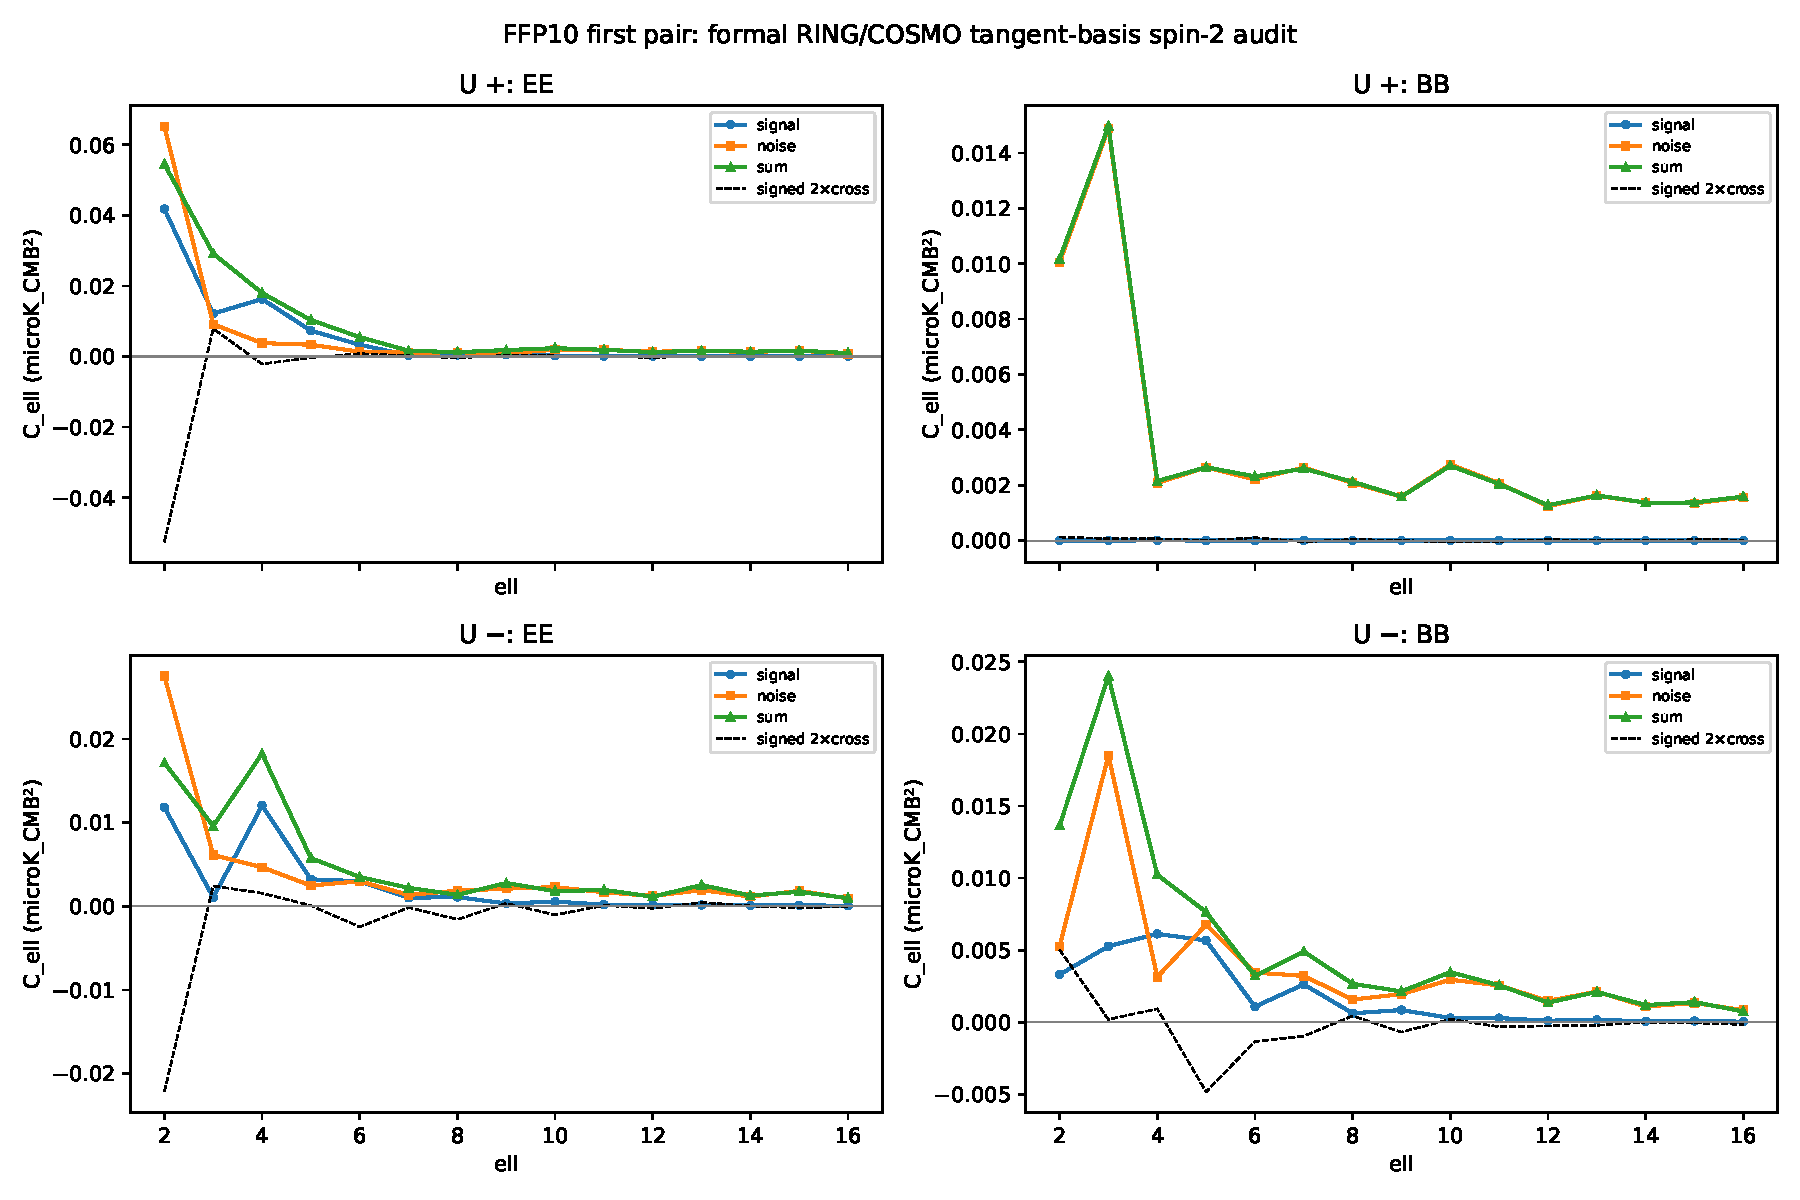
\includegraphics[width=\linewidth,height=.70\textheight,keepaspectratio]{../spectra_ffp10_first_pair_v1/diagnostic.pdf}
\caption{First raw pair formal spin-2 operator; U plus/minus are declared encodings; source bridge HOLD}
\end{figure}

\clearpage\begin{figure}[p]\centering
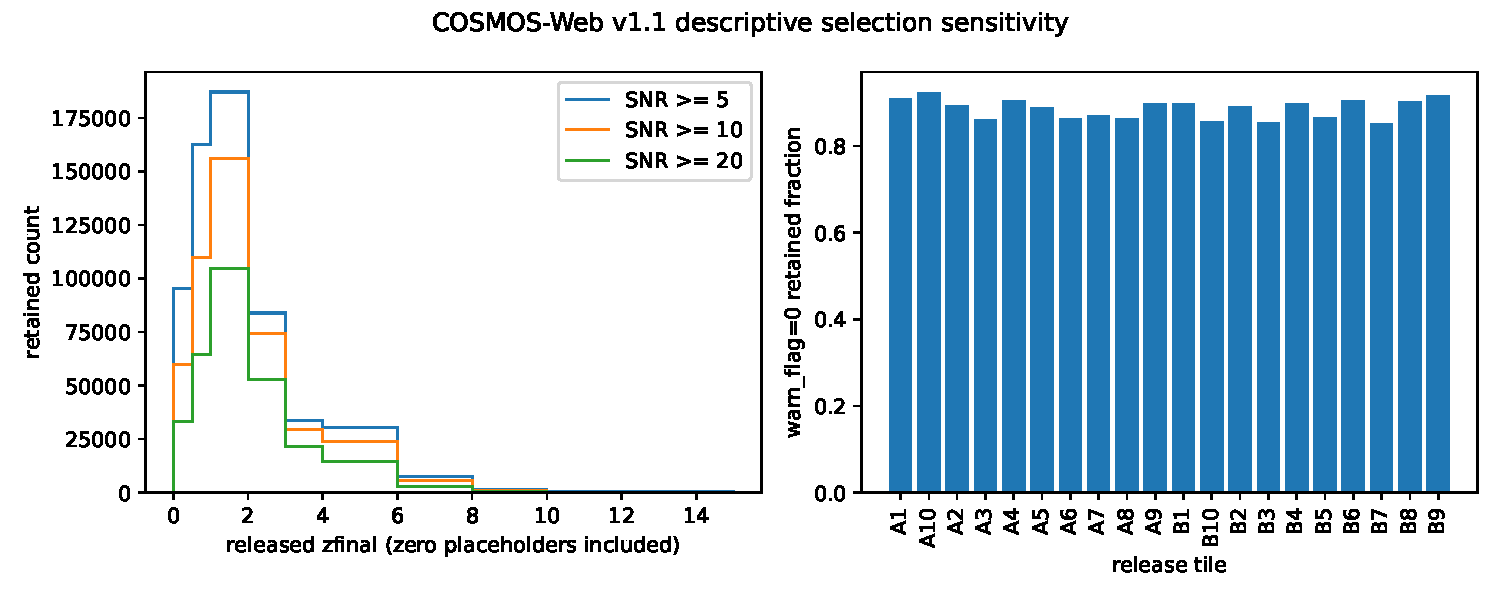
\includegraphics[width=\linewidth,height=.70\textheight,keepaspectratio]{../cosmos_selection_v1/selection_redshift.pdf}
\caption{Released zfinal retention includes zero star/artifact placeholders; no galaxy population or completeness inference}
\end{figure}

\clearpage\begin{figure}[p]\centering
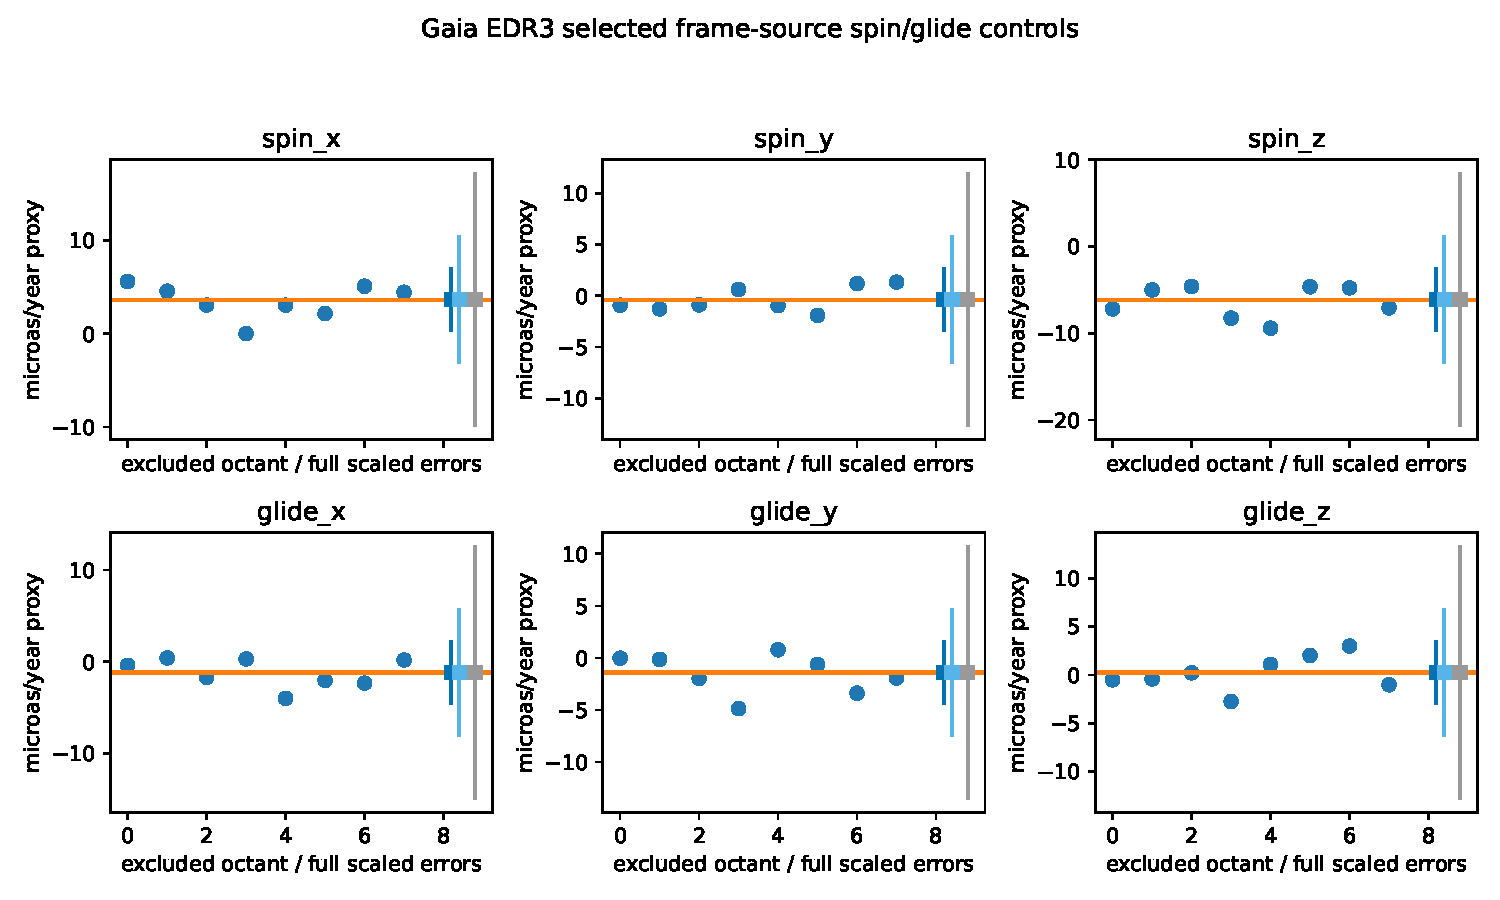
\includegraphics[width=\linewidth,height=.70\textheight,keepaspectratio]{../gaia_frame_v1/frame_controls.pdf}
\caption{4756 outcome-selected frame sources: spin/glide working model; no independent physics inference}
\end{figure}

\clearpage\begin{figure}[p]\centering
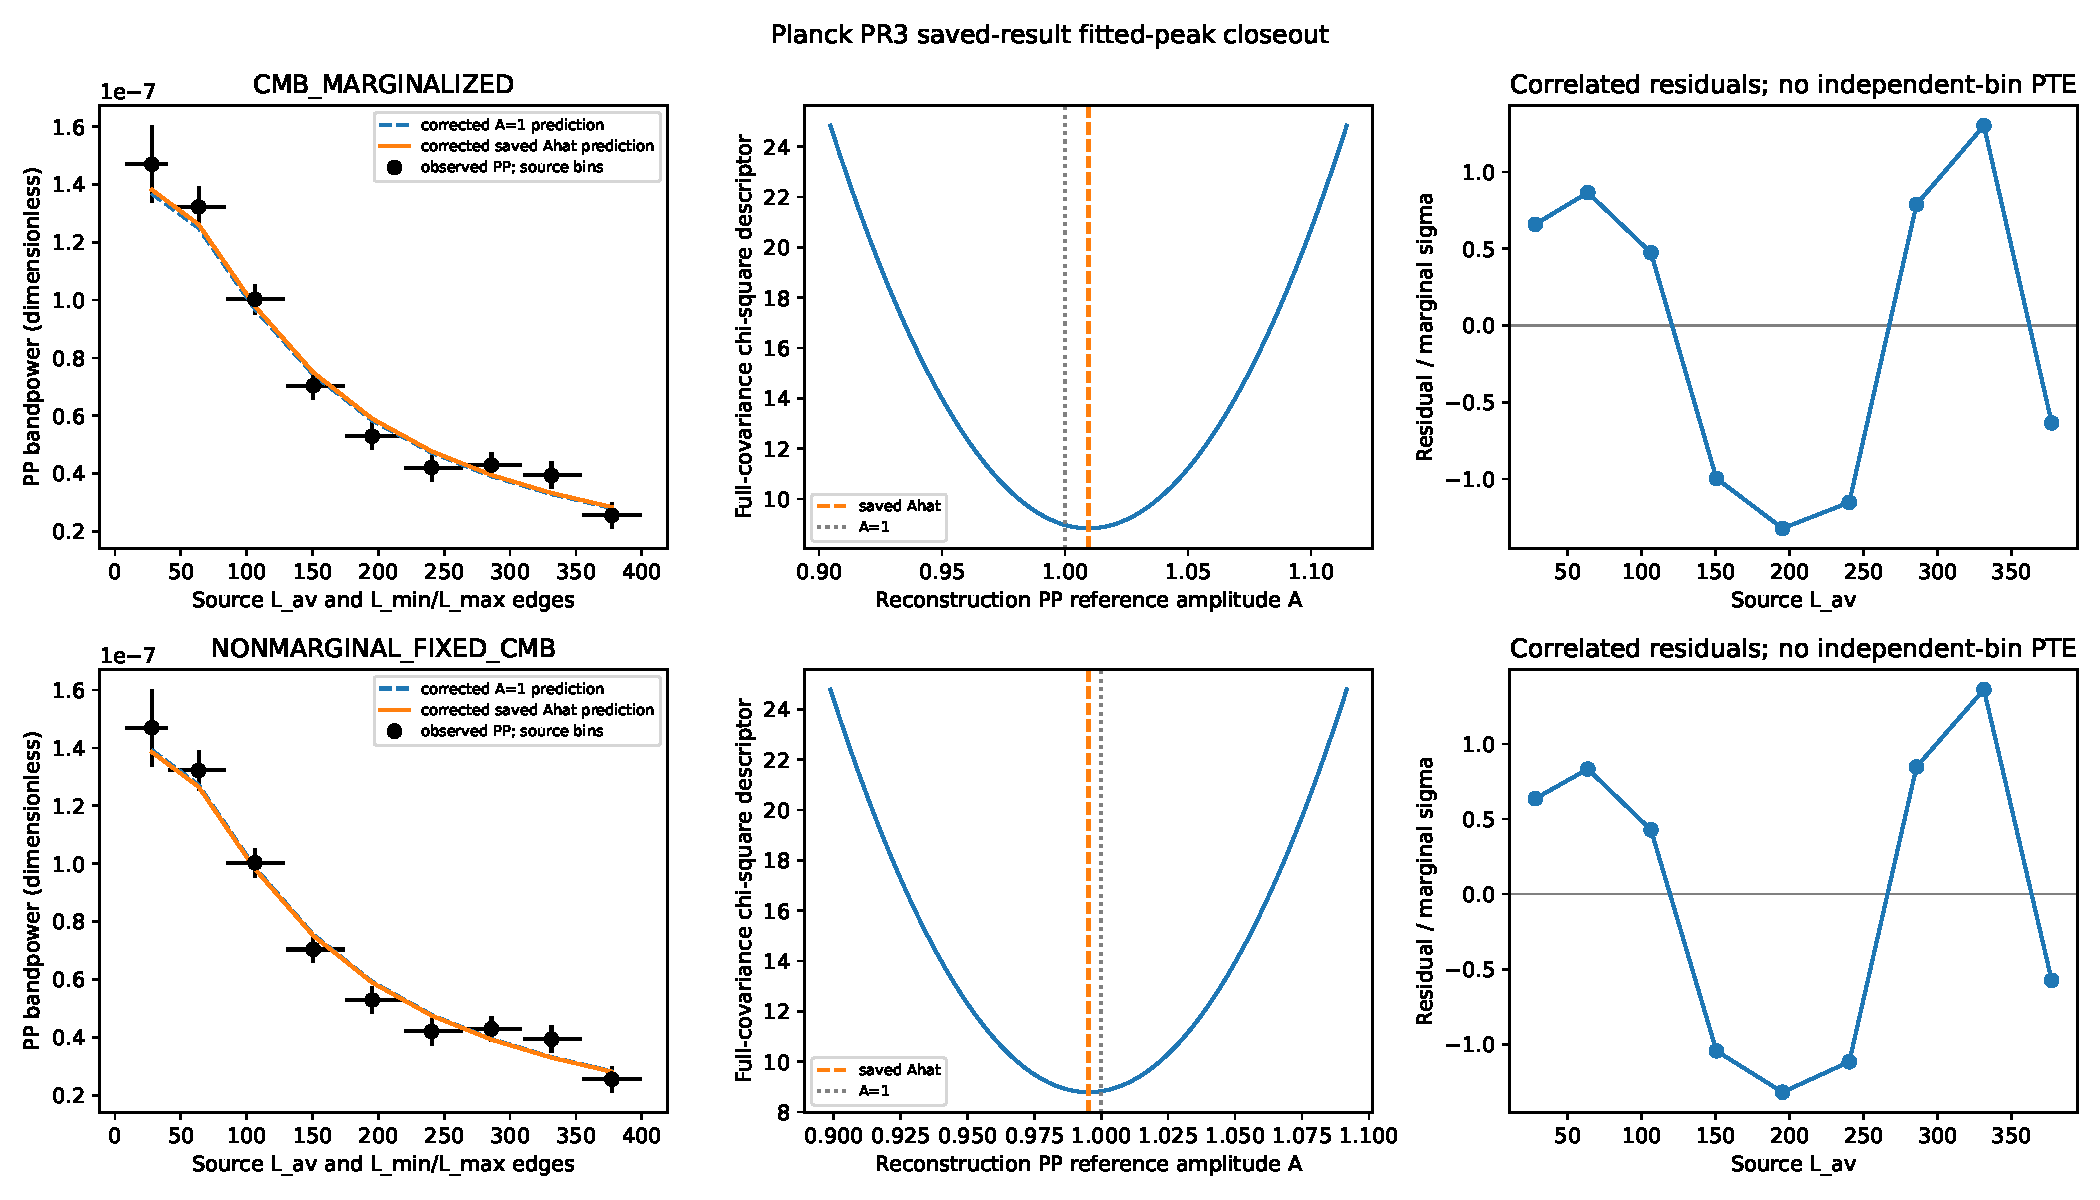
\includegraphics[width=\linewidth,height=.70\textheight,keepaspectratio]{../planck_pr3_peak_closeout_v1/peak_closeout.pdf}
\caption{Planck PR3 source-corrected reconstruction amplitude; shared Planck information retained}
\end{figure}
\end{document}
